\documentclass{beamer}
\usepackage{sdp}

\title{Редици}

\date{24 октомври 2017 г.}

\titlegraphicx{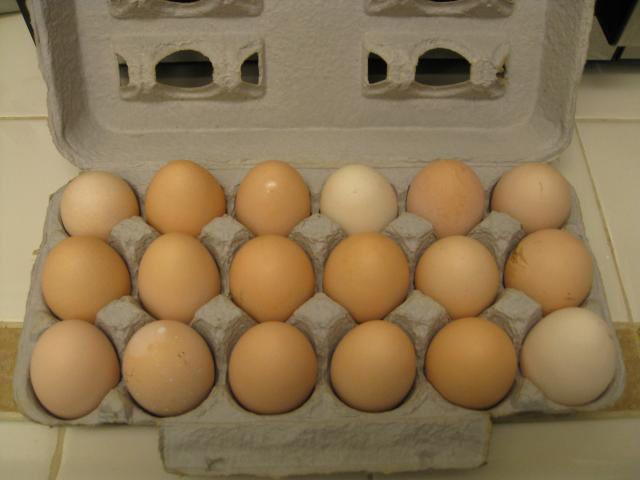
\includegraphics[height=0.25\textheight]{images/array.jpg}\\
  \imageBased{IMGP0612 - dozen eggs}{RaeAllen}{https://flic.kr/p/9vfsS}{CC BY-NC-SA 2.0}}

\begin{document}

\begin{frame}
  \titlepage
\end{frame}

\section{Масиви}

\begin{frame}
  \frametitle{АТД: Масив}

  Последователност от елементи от еднакъв вид, които могат да бъдат избирани по номер (индекс).\\[1em]\
  \pause
  \textbf{Операции}\\[0.5em]
  \begin{itemize}
  \item \lst{create(n)} --- създаване на масив със зададена големина
  \item \lst{get(i)} --- получаване на елемент с индекс \tt i
  \item \lst{set(i,x)} --- задаване на стойност \tt x на елемента с индекс \tt i
  \item \lst{size} --- дължина на масива
  \end{itemize}
  \vspace{1em}
  \pause
  \textbf{Свойства на операциите}\\[0.5em]
  \begin{itemize}
  \item \lst{a.set(i,x).get(i)} = \tt x
  \item \lst{a.set(i,x).get(j)} = \lst{a.get(j)}, ако \tt{i $\neq$ j}
  \item \lst{create(n).size} = \tt n
  \end{itemize}
\end{frame}

\begin{frame}
  \frametitle{Статично представяне}

  % TODO: да се нарисува с TikZ
  \begin{tabular}{|*8{c|}}
    \rowcolor{diagramblue}
    \hline
    $a_0$&$a_1$&$a_2$&\ldots&\ldots&\ldots&\ldots&$a_{n-1}$\\
    \hline
    \multicolumn{8}{c}{$\underbrace{\hspace{40ex}}_{\text{дължина}}$}\\
  \end{tabular}\\[3em]
  \textbf{Реализация:} масив във C++.\\[1em]
  \textbf{Пример:} \lst{int a[10];}
  % TODO: пример за операциите
\end{frame}

\begin{frame}
  \frametitle{Динамично представяне}
  \newcommand{\pha}{\hspace{2ex}}

  % TODO: да се нарисува с TikZ
  \begin{tabular}{|*{16}{c|}}
    \multicolumn{16}c{$\overbrace{\hspace{60ex}}^{\text{капацитет}}$}\\
    \rowcolor{diagramblue}
    \hline
    $a_0$&$a_1$&$a_2$&\ldots&\ldots&\ldots&\ldots&$a_{n-1}$&\pha&\pha&\pha&\pha&\pha&\pha&\pha&\pha\\
    \hline
    \multicolumn 8c{$\underbrace{\hspace{40ex}}_{\text{дължина}}$}&\multicolumn 8c{}
  \end{tabular}\\[3em]
  \textbf{Реализация:} \lst{std::vector}.
\end{frame}

\begin{frame}
  \frametitle{\lst{std::vector<T>}}

  Реализация на динамичен масив
  \begin{itemize}
  \item \lst{vector(n)} --- създава вектор с дължина \tt n
  \item \lst{size} --- дължина на вектора
  \item \lst{capacity} --- капацитет на вектора
  \item \lst{[i]}, \lst{at(i)} --- достъп до елемент на индекс \tt i
    % TODO: разлика между [] и at
  \item \lst{front()}, \lst{back()} --- достъп до първи и последен елемент
  \item \lst!push_back(x)! --- добавяне на елемента \tt x в края
  \item \lst!pop_back()! --- изтриване на последния елемент
  \item \lst{insert(...)} --- вмъкване на елементи на произволна позиция
  \item \lst{erase(...)} --- изтриване на елементи на произволна позиция
  \item \lst{==,!=,<,>,<=,>=} --- лексикорафско сравнение на два вектора
  \end{itemize}
  \pause
  Специализация \lst{vector<bool>}: реализирана чрез битови масиви
\end{frame}

\begin{frame}
  \frametitle{\lst{std::string}}

  Реализация на низ (динамична редица от символи)
  \begin{itemize}
  \item Всички методи на \lst{std::vector<char>}
    \begin{itemize}
    \item \alert{но не го наследява!}
    \end{itemize}
  \item Методите са съвместими с \lst{char*}
  \item \lst{replace(...)} --- подмяна на символи на произволна позиции
  \item \lst{+,+=,append(...)} --- конкатенация на низове
  \item \lst!<<, >>! --- операции за вход и изход
  \item \lst!c_str()! --- конвертиране към стандартен C++ низ
  \item \lst{find(...), rfind(...)} --- търсене на първо/последно срещане
  \item \lst!find_first_of(...)! --- първо срещане на символ от друг низ
  \item \lst{substr(...)} --- извличане на подниз
  \item \lst{compare(...)} --- сравнение с друг низ
  \item \lst{copy(...)} --- копиране на символи от C++ низ
  \end{itemize}
\end{frame}

\section{Кортежи}

\begin{frame}
  \frametitle{АТД: Наредена двойка}

  Двойка от елементи от потенциално различен тип, в която редът има значение.\\[0.5em]
  \textbf{Операции}\\[0.5em]
  \begin{itemize}
  \item \lst{create(a,b)} --- създава двойка от елементите \tt a и \tt b
  \item \lst{first} --- първият елемент на двойката
  \item \lst{second} --- вторият елемент на двойката
  \end{itemize}
  \vspace{0.5em}
  \textbf{Свойства на операциите}\\[0.5em]
  \begin{itemize}
  \item \lst{create(a,b).first} = \tt a
  \item \lst{create(a,b).second} = \tt b
  \item \lst{create(p.first,p.second)} = \tt p
  \end{itemize}
\end{frame}

\begin{frame}[fragile]
  \frametitle{Физическо представяне}

  % TODO: да се нарисува с TikZ
  \begin{center}
    \begin{tabular}{|m{5ex}|m{8ex}|}
      \hline
      \rowcolor{diagramblue}
      a&b\\
      \hline
    \end{tabular}
  \end{center}
  \vspace{2em}

  Възможни реализации:
  \begin{itemize}[<+->]
  \item \lst!struct Pair { int first; char second; };!
  \item \lst!std::pair<T,U>!
  \end{itemize}
\end{frame}

\begin{frame}
  \frametitle{\lst{std::pair}}

  Реализация на наредена двойка
  \begin{itemize}
  \item \lst{pair(x,y)} --- създаване на двойка (\tt x,\tt y)
  \item \lst{first} --- първи елемент
  \item \lst{second} --- втори елемент
  \item \lst{==,!=,<,>,<=,>=} --- лексикорафско сравнение на две двойки
  \end{itemize}
\end{frame}

\begin{frame}
  \frametitle{АТД: Кортеж}

  Редица от фиксиран брой елементи от потенциално различен тип, в която редът има значение.\\[0.5em]

  \textbf{Операции}\\[0.5em]
  \begin{itemize}
  \item \lst{create(...)} --- създаване на кортеж по единични елементи
  \item \lst{get(i)} --- получаване на елемент с индекс/име \tt i
  \item \lst{set(i,x)} --- задаване на стойност \tt x на елемента с индекс/име \tt i
  \end{itemize}

  \textbf{Свойства на операциите}\\[0.5em]
  \begin{itemize}
  \item \tt{create(a$_1$,\ldots,a$_i$,\ldots,a$_n$).get(i)} = \tt{a$_i$}
  \item \lst{t.set(i,x).get(i)} = \tt x
  \item \lst{t.set(i,x).get(j)} = \lst{a.get(j)}, ако \tt{i $\neq$ j}
  \end{itemize}
\end{frame}

\begin{frame}
  \frametitle{\lst{std::tuple} (C++11)}

  Реализация на кортеж
  \begin{itemize}
  \item \lst{tuple(...)} --- създаване на кортеж с подадените елементи
  \item \lst!tuple_cat(...)! --- слепва произволен брой кортежи
  \item \lst{get(i)} --- $i$-ти елемент на кортежа
  \item \lst {==,!=,<,>,<=,>=} --- лексикорафско сравнение на два кортежа
  \end{itemize}
\end{frame}


\end{document}
